\documentclass[]
{UCD_CS_41820_Report}
\usepackage{graphicx}
\usepackage{listings}
\usepackage{xcolor}


\definecolor{codegreen}{rgb}{0,0.6,0}
\definecolor{codegray}{rgb}{0.5,0.5,0.5}
\definecolor{codepurple}{rgb}{0.58,0,0.82}
\definecolor{backcolour}{rgb}{0.95,0.95,0.92}
\usepackage{color}
\definecolor{lightgray}{rgb}{0.95, 0.95, 0.95}
\definecolor{darkgray}{rgb}{0.4, 0.4, 0.4}
%\definecolor{purple}{rgb}{0.65, 0.12, 0.82}
\definecolor{editorGray}{rgb}{0.95, 0.95, 0.95}
\definecolor{editorOcher}{rgb}{1, 0.5, 0} % #FF7F00 -> rgb(239, 169, 0)
\definecolor{editorGreen}{rgb}{0, 0.5, 0} % #007C00 -> rgb(0, 124, 0)
\definecolor{orange}{rgb}{1,0.45,0.13}		
\definecolor{olive}{rgb}{0.17,0.59,0.20}
\definecolor{brown}{rgb}{0.69,0.31,0.31}
\definecolor{purple}{rgb}{0.38,0.18,0.81}
\definecolor{lightblue}{rgb}{0.1,0.57,0.7}
\definecolor{lightred}{rgb}{1,0.4,0.5}
\usepackage{upquote}
\usepackage{textcomp}
\usepackage{float}
\setcounter{secnumdepth}{3}



% CSS
\lstdefinelanguage{CSS}{
  keywords={color,background-image:,margin,padding,font,weight,display,position,top,left,right,bottom,list,style,border,size,white,space,min,width, transition:, transform:, transition-property, transition-duration, transition-timing-function},	
  sensitive=true,
  morecomment=[l]{//},
  morecomment=[s]{/*}{*/},
  morestring=[b]',
  morestring=[b]",
  alsoletter={:},
  alsodigit={-}
}

% JavaScript
\lstdefinelanguage{JavaScript}{
  morekeywords={typeof, new, true, false, catch, function, return, null, switch, var, let, const, if, in, while, do, else, case, break, await, async},
  morecomment=[s]{/*}{*/},
  morecomment=[l]//,
  morestring=[b]",
  morestring=[b]',
  morestring=[b]`,
  literate={\$}{{$$$$}}1
}




\lstdefinelanguage{HTML5}{
  language=html,
  sensitive=true,	
  alsoletter={<>=-},	
  morecomment=[s]{<!-}{-->},
  tag=[s],
  otherkeywords={
  % General
  >,
  % Standard tags
	<!DOCTYPE,
  </html, <html, <head, <title, </title, <style, </style, <link, </head, <meta, />,
	% body
	</body, <body,
	% Divs
	</div, <div, </div>, 
	% Paragraphs
	</p, <p, </p>,
	% scripts
	</script, <script,
  % More tags...
  <canvas, /canvas>, <svg, <rect, <animateTransform, </rect>, </svg>, <video, <source, <iframe, </iframe>, </video>, <image, </image>, <header, </header, <article, </article
  },
  ndkeywords={
  % General
  =,
  % HTML attributes
  charset=, src=, id=, width=, height=, style=, type=, rel=, href=,
  % SVG attributes
  fill=, attributeName=, begin=, dur=, from=, to=, poster=, controls=, x=, y=, repeatCount=, xlink:href=,
  % properties
  margin:, padding:, background-image:, border:, top:, left:, position:, width:, height:, margin-top:, margin-bottom:, font-size:, line-height:,
	% CSS3 properties
  transform:, -moz-transform:, -webkit-transform:,
  animation:, -webkit-animation:,
  transition:,  transition-duration:, transition-property:, transition-timing-function:,
  }
}

\lstdefinestyle{htmlcssjs} {%
  % General design
%  backgroundcolor=\color{editorGray},
  basicstyle={\footnotesize\ttfamily},   
  frame=b,
  % line-numbers
  xleftmargin={0.75cm},
  numbers=left,
  stepnumber=1,
  firstnumber=1,
  numberfirstline=true,	
  % Code design
  identifierstyle=\color{black},
  keywordstyle=\color{blue}\bfseries,
  ndkeywordstyle=\color{editorGreen}\bfseries,
  stringstyle=\color{editorOcher}\ttfamily,
  commentstyle=\color{brown}\ttfamily,
  % Code
  language=HTML5,
  alsolanguage=JavaScript,
  alsodigit={.:;},	
  tabsize=2,
  showtabs=false,
  showspaces=false,
  showstringspaces=false,
  extendedchars=true,
  breaklines=true,
  % German umlauts
  literate=%
  {Ö}{{\"O}}1
  {Ä}{{\"A}}1
  {Ü}{{\"U}}1
  {ß}{{\ss}}1
  {ü}{{\"u}}1
  {ä}{{\"a}}1
  {ö}{{\"o}}1
}
%
\lstdefinestyle{py} {%
language=python,
literate=%
*{0}{{{\color{lightred}0}}}1
{1}{{{\color{lightred}1}}}1
{2}{{{\color{lightred}2}}}1
{3}{{{\color{lightred}3}}}1
{4}{{{\color{lightred}4}}}1
{5}{{{\color{lightred}5}}}1
{6}{{{\color{lightred}6}}}1
{7}{{{\color{lightred}7}}}1
{8}{{{\color{lightred}8}}}1
{9}{{{\color{lightred}9}}}1,
basicstyle=\footnotesize\ttfamily, % Standardschrift
numbers=left,               % Ort der Zeilennummern
%numberstyle=\tiny,          % Stil der Zeilennummern
%stepnumber=2,               % Abstand zwischen den Zeilennummern
numbersep=5pt,              % Abstand der Nummern zum Text
tabsize=4,                  % Groesse von Tabs
extendedchars=true,         %
breaklines=true,            % Zeilen werden Umgebrochen
keywordstyle=\color{blue}\bfseries,
frame=b,
commentstyle=\color{brown}\itshape,
stringstyle=\color{editorOcher}\ttfamily, % Farbe der String
showspaces=false,           % Leerzeichen anzeigen ?
showtabs=false,             % Tabs anzeigen ?
xleftmargin=17pt,
framexleftmargin=17pt,
framexrightmargin=5pt,
framexbottommargin=4pt,
%backgroundcolor=\color{lightgray},
showstringspaces=false,      % Leerzeichen in Strings anzeigen ?
}%
%

\lstdefinestyle{mystyle}{
    backgroundcolor=\color{backcolour},   
    commentstyle=\color{codegreen},
    keywordstyle=\color{magenta},
    numberstyle=\tiny\color{codegray},
    stringstyle=\color{codepurple},
    basicstyle=\ttfamily\footnotesize,
    breakatwhitespace=false,         
    breaklines=true,                 
    captionpos=b,                    
    keepspaces=true,                 
    numbers=left,                    
    numbersep=5pt,                  
    showspaces=false,                
    showstringspaces=false,
    showtabs=false,                  
    tabsize=2
}

\lstset{style=htmlcssjs}
\usepackage{hyperref}
\hypersetup{
    colorlinks=true,
    linkcolor=blue,
    filecolor=magenta,      
    urlcolor=cyan,
}
\lstset{
    mathescape=true,
    basicstyle = \ttfamily
}


%\usepackage[backend=biber,style=chicago-authordate]{biblatex}
\usepackage[backend=biber,style=nature]{biblatex}
\addbibresource{references.bib}


%%% YOU DO NOT NEED TO EDIT ANYTHING ABOVE THIS LINE
%%% START EDITING THE DOCUMENT BELOW
%%%%%%%%%%%%%%%%%%%%%%
%%% Input project details

\def\firststudentname{Pelayo García Álvarez}% Edit with your name
\def\firststudentid{25236718}% Edit with your student id
\def\secondstudentname{José Ramón Morera Campos}% Edit with your name
\def\secondstudentid{25248785}% Edit with your student id
\def\projecttitle{CitySwift (Network Optimization for Bus Éireann Dublin)} % Edit with your project title
\def\supervisorname{Vivek Nallur}


\begin{document}
\maketitle

%%%%%%%%%%%%%%%%%%%%%%
%%% Table of Content

\tableofcontents
%\pdfbookmark[0]{Table of Contents}{toc}\newpage
%\newpage


%%%%%%
\chapter{Introduction}
The integration of artificial intelligence into public infrastructure represents a fundamental paradigm shift in urban mobility, transitioning societies from reactive transit management to predictive, algorithmic governance. This report provides an exhaustive ethical and socio-technical evaluation of a real-world, deployed artificial intelligence system: the CitySwift Performance Optimisation Platform, specifically analyzing its integration within the Bus Éireann network and wider public transport franchising models \cite{cityswift_bus_eireann}.

Functioning as an intelligent transport data platform, the system ingests immense volumes of enriched network performance data to deliver predictive analytics, automated scheduling, and real-time operational optimization. By optimizing over 3.3 billion passenger journeys annually across the globe \cite{galwaybayfm_cityswift} and processing vast histories of enriched network performance data, the platform acts as the central algorithmic nervous system for transport operators and municipal authorities. The system features a sophisticated suite of specialized modules—including the Data Engine, Discover, Evolve, and Explore—that facilitate continuous scenario planning, resource modeling, and the rigorous optimization of bus network runtimes \cite{cityswift_gov_uk}.

\section*{Key Features}
A critical analytical vector for understanding the CitySwift system lies in identifying its underlying artificial intelligence architecture. While public-facing documentation relies on generalized terminology such as "intelligent recommendations" and "AI-powered analytics," there is no public evidence explicitly confirming the exact algorithmic taxonomy used under the hood. Therefore, we present our \textbf{best guess}, with plausible justification, that CitySwift operates as an advanced hybrid neuro-symbolic system. This architecture purposefully leverages both symbolic and sub-symbolic artificial intelligence methodologies to bridge the knowledge acquisition bottleneck while maintaining logical, contractual oversight \cite{intro_machine_ethics}.

\textbf{Sub-Symbolic AI:} Sub-symbolic artificial intelligence, which encompasses connectionism, deep learning, and probabilistic machine learning models, excels in pattern recognition, high-dimensional scalability, and the handling of massive, noisy datasets. CitySwift's core capacity to process millions of Automatic Vehicle Location (AVL) data pings daily, analyze erratic ticketing anomalies, and forecast complex origin-destination passenger flows heavily implies the foundational use of sub-symbolic architectures. These machine learning models operate probabilistically, predicting future transit demand, simulating complex network interactions within the \textit{Evolve} module, and anticipating traffic congestion delays based on historical variables. However, sub-symbolic artificial intelligence inherently suffers from a lack of transparency and interpretability, often functioning as a computational "black box" where tracing the exact decision-making process becomes mathematically intractable for human auditors.

\textbf{Symbolic AI:} To counteract this architectural opacity, we hypothesize—again, as a \textbf{best guess} since proprietary code is unavailable—that the platform simultaneously employs symbolic artificial intelligence. Symbolic AI encompasses rule-based systems, explicit logic programming, and expert systems characterized by their reliance on human-readable logic \cite{intro_prop_logic}. Symbolic AI handles structured logical problems and provides the exact transparency required for contractual and financial accountability in public sector deployments. We guess that this is most evident in the platform's incident management protocol and delay categorization logic. When a transit disruption occurs, the system likely utilizes an explicit, rule-based categorization matrix (a symbolic expert system) to determine if a delay is "operator-controlled" (e.g., driver error or fleet maintenance failure) or "externally-controlled" (e.g., unexpected infrastructure bottlenecks or severe weather events).

\begin{table}[h!]
  \centering
  \begin{tabular}{|p{3.2cm}|p{3.5cm}|p{3.5cm}|p{4cm}|}
    \hline
    \textbf{AI Methodology}                                                                                                                 & \textbf{Core Strengths} & \textbf{Inherent Weaknesses} & \textbf{CitySwift Platform Application} \\
    \hline
    \textbf{Sub-Symbolic AI} \newline (Machine Learning, Neural Networks)                                                                   &
    Unmatched pattern recognition, scalability across billions of data points, adaptability to noisy, unstructured AVL telemetry.           &
    Severe lack of transparency, interpretability issues, highly susceptible to hidden historical data biases, operates as a black box.     &
    Powers the predictive forecasting engines, demand analysis tools, and the simulation capabilities of the Evolve module.                                                                                                                    \\
    \hline
    \textbf{Symbolic AI} \newline (Rule-Based Systems, Expert Systems)                                                                      &
    Explicit logical reasoning, complete transparency, highly effective for structured regulatory problems, requires minimal training data. &
    Extreme inflexibility, suffers from the knowledge acquisition bottleneck, highly brittle when processing unexpected edge cases.         &
    \textit{(Best Guess)} Drives the incident management system, administers the operator vs. externally-controlled categorization logic, and ensures contractual compliance.                                                                  \\
    \hline
  \end{tabular}
  \caption{Comparison of AI Methodologies within the CitySwift Architecture}
\end{table}

This hypothesized neuro-symbolic integration represents a highly sophisticated socio-technical achievement. A sub-symbolic neural component continuously processes raw environmental data to predict network realities, while a symbolic component applies rigid contractual logic to these predictions, allowing the platform to deliver data-led decisions with a high degree of operational confidence.

\section*{1.1 Functional Goals of the System}
As documented in CitySwift's service definitions and its public partnership announcements with Bus Éireann \cite{cityswift_bus_eireann, cityswift_gov_uk}, the platform moves beyond generic data visualization to achieve highly specific, operational goals explicitly engineered to maximize network efficiency, operational predictability, and data integrity. The concrete functional objectives of the deployed system are:

\begin{itemize}
  \item \textbf{High-Fidelity Telemetry Fusion:} To continuously ingest and reconcile disparate, high-frequency transit data streams—specifically Automatic Vehicle Location (AVL) GPS pings, Real-Time Passenger Information (RTPI), and electronic ticketing logs. This creates a singular, "cleansed" record of truth, preventing historical data noise from polluting newly franchised operational models.

  \item \textbf{Automated Delay Causality Categorization:} To calculate micro-metrics like Excess Wait Time (EWT) and stop-specific dwell times. \textit{(Best Guess)} The system functionally aims to flag whether a delay is "Operator-Controlled" or "Externally-Controlled" via a rule-based categorization matrix, which serves as the evidentiary basis for contractual financial adjustments between authorities and operators.

  \item \textbf{Risk-Aware Schedule Simulation:} To utilize sub-symbolic machine learning models within the \textit{Evolve} module to simulate the impact of proposed timetable adjustments \textit{in silico}. This allows planners to statistically evaluate the trade-off between reducing vehicle "slack time" (efficiency) and the risk of late running (reliability).

  \item \textbf{Dynamic Demand-Capacity Matching:} To analyze passenger movement patterns to predict future trends and identify emerging mobility opportunities. The system aims to dynamically adjust headways to eradicate "bus bunching" during peak hours, ensuring that vehicle capacity is distributed precisely where and when demand is highest.

  \item \textbf{Operational Resource Optimization:} To maximize the utilization of the network’s finite vehicular resources. By optimizing active fleet distribution and driver shift patterns, the system functionally minimizes "dead mileage" (non-revenue travel), reducing unnecessary fuel consumption and the overall carbon footprint per passenger journey.

  \item \textbf{Multi-Stakeholder Performance Transparency:} To provide automated, standardized reporting interfaces for different actors (regulators, operators, and planners). This goal ensures that all stakeholders have simultaneous access to the same performance KPIs, facilitating rapid incident management and objective performance audits.

  \item \textbf{Accessibility and Service-Reliability Analysis:} To identify specific network vulnerabilities where service gaps or chronic unreliability disproportionately affect certain routes. The functional goal is to provide data-driven evidence that allows for the protection of transit-dependent communities through targeted service interventions.
\end{itemize}


%%%%%%%%
\chapter{Stakeholder Identification}
The deployment of an autonomous predictive algorithmic platform across a national public transport network introduces a vast, interconnected matrix of stakeholders. To systematically identify these actors and the ethical boundaries of their interactions, we apply the STEEPL (Social, Technical, Economic, Ecological, Political, Legal) framework.

Crucially, the primary actors in this ecosystem—most notably the transit operators, engineers, and commuters—operate under a strict functional-to-ethical goals ratio of at least 5:1. As established in Section 1.1, the system exists fundamentally to execute five primary functional goals: data integration, runtime forecasting, schedule optimization, \textit{in silico} simulation, and delay categorization. The sheer volume of these functional goals dictates the system's computational priorities. However, to operate safely and fairly, each primary stakeholder category is constrained by at least one overarching ethical goal. While these ethical goals do not overshadow the functional objectives in number, they present significantly more complex challenges regarding logical implementation and regulatory compliance.

Below is the identification of the primary and secondary actors within the STEEPL categories, alongside their corresponding ethical principles and the philosophical schools of thought that govern them.

\begin{table}[H]
  \centering
  \renewcommand{\arraystretch}{1.5}
  \begin{tabular}{|p{1.7cm}|p{3.7cm}|p{3.5cm}|p{4.5cm}|}
    \hline
    \textbf{STEEPL Category}                                                                                                      &
    \textbf{Stakeholders (Primary \& Secondary)}                                                                                  &
    \textbf{Dominant Ethical Principle (The "1" in 5:1)}                                                                          &
    \textbf{Applicable School(s) of Ethical Thought}                                                                                                                                                                    \\
    \hline

    \textbf{Social}                                                                                                               &
    \textbf{Primary:} Commuters \& Passengers \newline
    \textbf{Secondary:} Transit Advocacy Groups                                                                                   &
    \textbf{Equitable Access:} Preventing the algorithmic creation of "transit deserts" for vulnerable populations.               &
    \textbf{Relational Ethics / Ethics of Care:} Prioritizes the societal bond and the moral obligation to care for marginalized communities who rely heavily on public infrastructure \cite{relational_ethics}.        \\
    \hline

    \textbf{Technical}                                                                                                            &
    \textbf{Primary:} CitySwift Engineers \newline
    \textbf{Secondary:} Bus Éireann IT Admin                                                                                      &
    \textbf{Transparency:} Ensuring the system's logic is verifiable and not an opaque "black box."                               &
    \textbf{Deontology:} The engineer has a strict professional duty (rule-based ethics) to ensure safety constraints are formally verifiable and logically sound \cite{intro_machine_ethics}.                          \\
    \hline

    \textbf{Economic}                                                                                                             &
    \textbf{Primary:} Transit Operators (Bus Éireann) \newline
    \textbf{Secondary:} Taxpayers / Investors                                                                                     &
    \textbf{Fairness in Penalties:} Ensuring algorithmic categorizations of delays do not result in unjust financial penalties.   &
    \textbf{Utilitarianism vs. Deontology:} Utilitarianism drives the functional goal of maximizing network profitability, but it must be constrained by the Deontological right to fair, auditable contract execution. \\
    \hline

    \textbf{Ecological}                                                                                                           &
    \textbf{Primary:} Local Urban Residents \newline
    \textbf{Secondary:} Environmental Protection Agencies                                                                         &
    \textbf{Harm Reduction:} Minimizing the physical carbon footprint and particulate emissions of the bus fleet.                 &
    \textbf{Virtue Ethics:} Evaluated by the "character" of the institutional agent—demonstrating corporate virtue by actively prioritizing environmental stewardship over sheer operational throughput.                \\
    \hline

    \textbf{Political}                                                                                                            &
    \textbf{Primary:} National Transport Authority (NTA) \newline
    \textbf{Secondary:} Department of Transport                                                                                   &
    \textbf{Accountability:} Ensuring algorithmic sovereignty does not usurp the state's responsibility for civic infrastructure. &
    \textbf{Deontology:} The state holds an absolute, non-transferable duty to provide safe, equitable civic services to its citizens, regardless of the technological mediators used.                                  \\
    \hline

    \textbf{Legal}                                                                                                                &
    \textbf{Primary:} Bus Drivers (Subject to tracking) \newline
    \textbf{Secondary:} Data Protection Officers (DPOs)                                                                           &
    \textbf{Right to Privacy:} Protecting employee and passenger telemetry from unwarranted surveillance or misuse (GDPR).        &
    \textbf{Deontology:} Strict, rule-based adherence to legal frameworks and human rights, asserting that individuals are ends in themselves, not merely data points for algorithmic optimization.                     \\
    \hline
  \end{tabular}
  \caption{STEEPL Stakeholder Identification and Ethical Mapping}
\end{table}

\section*{2.1 Ethical Goals of the System}
When evaluating the publicly stated ethical goals of the CitySwift platform, a critical distinction must be made between the corporate ethics of the company and the codified ethical goals of the algorithmic system itself. As is common in commercial AI deployments, \textbf{there are almost no explicitly stated ethical goals for the algorithmic system itself} within its technical or public-facing documentation; the system's documented parameters are overwhelmingly functional (e.g., maximizing throughput, minimizing dwell time) \cite{cityswift_gov_uk}.

However, at the corporate level, the organization heavily emphasizes environmental sustainability and institutional transparency. CitySwift's most prominent ethical commitment is its Climate Action Policy, which formalizes a vision to reduce global transport emissions. The company states that it is effectively Net Zero based on the carbon savings delivered by its platform and targets a cumulative reduction of 100 million kilograms of carbon dioxide by 2030 \cite{cityswift_esg}. Furthermore, the company explicitly champions the creation of a "single source of truth" to replace adversarial operator-authority relationships with transparent, data-driven collaboration. Internally, the organization publishes a Gender Pay Gap Report and enforces an Anti-slavery and Human Trafficking Policy \cite{cityswift_esg}. Yet, it must be documented that these represent human corporate governance rather than formalized, machine-readable ethical constraints explicitly programmed into the system's state space \cite{intro_machine_ethics}.

\section*{2.2 Ethical Considerations}
To critically evaluate the behavioral parameters of the CitySwift platform, three distinct schools of ethical thought discussed in the module—Utilitarianism, Deontology, and Virtue Ethics—are applied as a candidate pool \cite{intro_machine_ethics}. Using the stakeholders identified in Chapter 2, we establish the major ethical goals of the system under each school and dictate how the system ought to behave.

\subsection*{2.2.1 Utilitarianism: Network Optimization and Distributive Justice}
\textbf{Major Ethical Goal:} To maximize aggregate network efficiency and passenger utility without inadvertently creating algorithmic transit deserts for marginalized communities (Stakeholders: Commuters \& Passengers, Transit Advocacy Groups).

\begin{itemize}
  \item \textbf{Relevant Variables:} Passenger demand volume (tap-ons), excess wait time (EWT), fleet utilization rates, and demographic transit-reliance indices for specific origin-destination flows.
  \item \textbf{System Functionality:} The \textit{Evolve} module ingests historical Automatic Vehicle Location (AVL) and ticketing data to simulate scheduling scenarios, dynamically calculating which configuration yields the highest ratio of successful passenger journeys to operational fuel costs.
  \item \textbf{What the System Will Do (or Not):} The system \textbf{will not} be permitted to dynamically reallocate the entirety of the fleet away from low-density, rural, or economically deprived routes simply because high-density urban corridors offer mathematically higher aggregate throughput. The system \textbf{will} enforce a "minimum service baseline" constraint across all routes, regardless of raw profitability or volume.
  \item \textbf{Relevant Ethical Principle cited:} This decision applies \textbf{Rule Utilitarianism} combined with the principle of \textbf{Distributive Justice} \cite{intro_machine_ethics}. While strict Act Utilitarianism would ruthlessly cut low-volume routes to maximize overall network numbers, Rule Utilitarianism recognizes that establishing a rule guaranteeing basic mobility access for all demographics ultimately generates greater long-term societal utility and trust in public infrastructure.
\end{itemize}

\subsection*{2.2.2 Deontology: Algorithmic Sovereignty and Contractual Fairness}
\textbf{Major Ethical Goal:} To ensure that automated financial penalties and delay categorizations are verifiable, respecting the fundamental right to transparent due process (Stakeholders: Transit Operators, CitySwift Engineers, DPOs).

\begin{itemize}
  \item \textbf{Relevant Variables:} Delay location coordinates, incident categorization flags (operator vs. external), traffic congestion telemetry, and financial penalty multipliers.
  \item \textbf{System Functionality:} The system automatically processes timing anomalies and applies a categorization matrix to determine the root cause of network friction (e.g., driver error vs. heavy traffic), reporting this to the franchising authority to enforce Service Level Agreements (SLAs).
  \item \textbf{What the System Will Do (or Not):} The system \textbf{will not} issue a definitive "operator-controlled" delay categorization if the underlying machine learning prediction falls below a 95\% confidence threshold, nor will it rely solely on sub-symbolic "black box" neural networks for this classification. The system \textbf{will} fallback to a human-in-the-loop audit trigger if the delay cannot be explicitly mapped using human-readable symbolic logic.
  \item \textbf{Relevant Ethical Principle cited:} This decision is grounded in the \textbf{Deontological Duty of Transparency and Fairness} \cite{intro_machine_ethics}. Deontology dictates that individuals and organizations must not be treated merely as a means to an end (in this case, streamlined municipal reporting). The operator holds a strict right to auditable fairness; therefore, the system has a categorical imperative to ensure its punitive outputs are hermeneutically reverse-engineerable.
\end{itemize}

\subsection*{2.2.3 Virtue Ethics: Ecological Character vs. The Ethics of Care}
\textbf{Major Ethical Goal:} To embody the virtues of environmental stewardship while simultaneously maintaining the virtue of compassion for vulnerable human passengers (Stakeholders: Local Urban Residents, Commuters).

\begin{itemize}
  \item \textbf{Relevant Variables:} Kilograms of $CO_{2}$ emissions saved, route energy efficiency indices, dead-mileage metrics, and passenger wait-time during severe weather conditions.
  \item \textbf{System Functionality:} The platform incorporates carbon output parameters into its optimization algorithms, recommending timetable adjustments and fleet distributions that drastically reduce fuel consumption and non-revenue-generating idling times.
  \item \textbf{What the System Will Do (or Not):} The system \textbf{will} optimize for absolute minimum fuel consumption and carbon output during standard operational parameters. However, the system \textbf{will not} enforce strict anti-idling or extended headway (wait time) optimizations during extreme weather events (e.g., freezing temperatures or severe storms). During these events, the system \textbf{will} prioritize rapid passenger boarding and vehicle climate-control allowances over marginal carbon savings.
  \item \textbf{Relevant Ethical Principle cited:} This decision utilizes \textbf{Virtue Ethics}, specifically balancing the virtue of \textbf{Ecological Stewardship} with the \textbf{Virtue of Care/Compassion} \cite{relational_ethics}. An ethically virtuous autonomous agent must possess practical wisdom (\textit{phronesis}); it recognizes that while environmental conservation is a profound virtue, rigidly optimizing for carbon reduction at the expense of leaving passengers exposed to hazardous conditions demonstrates a lack of holistic institutional character.
\end{itemize}

\section*{2.3 Values}

The introduction of the CitySwift predictive platform into the Bus Éireann network forces a convergence of disparate stakeholder values. To ensure the system operates ethically, we must explicitly map these values, analyze their alignment with our chosen ethical frameworks, and establish a hierarchy for algorithmic negotiation.

\subsection*{Stakeholder Values and Ethical Alignment}
Building upon the STEEPL framework established in Section 2.1, the core values of the primary stakeholders align with our ethical schools of thought as follows:

\paragraph{Commuters \& Passengers (Social)}
\begin{itemize}
  \item \textbf{Values:} Reliability, affordable mobility, safety, and equitable access to the network regardless of geographic location.
  \item \textbf{Ethical Alignment:} Strongly aligns with Relational Ethics and Distributive Justice, demanding that vulnerable or rural populations are not mathematically marginalized by the algorithm.
\end{itemize}

\paragraph{CitySwift Engineers (Technical)}
\begin{itemize}
  \item \textbf{Values:} Technical innovation, predictive accuracy, and system verifiability.
  \item \textbf{Ethical Alignment:} Aligns with Deontology, as engineers possess a professional duty to ensure the system’s logic is transparent and not an unaccountable ``black box''.
\end{itemize}

\paragraph{Transit Operators / Bus Éireann (Economic)}
\begin{itemize}
  \item \textbf{Values:} Maximized throughput, resource efficiency, cost reduction, and fairness in algorithmic penalty application.
  \item \textbf{Ethical Alignment:} Driven fundamentally by Utilitarianism (maximizing network utility/profit), but constrained by the Deontological right to fair, transparent contract execution regarding delay categorizations.
\end{itemize}

\paragraph{Local Urban Residents (Ecological)}
\begin{itemize}
  \item \textbf{Values:} Clean air, reduced particulate emissions, and environmental sustainability.
  \item \textbf{Ethical Alignment:} Reflects Virtue Ethics, specifically the virtue of ecological stewardship and harm reduction.
\end{itemize}

\paragraph{National Transport Authority / NTA (Political)}
\begin{itemize}
  \item \textbf{Values:} The public good, infrastructural accountability, and civic duty.
  \item \textbf{Ethical Alignment:} Anchored in Deontology, asserting the state's non-transferable obligation to provide safe civic services.
\end{itemize}

\paragraph{Bus Drivers (Legal)}
\begin{itemize}
  \item \textbf{Values:} Workplace fairness, job security, and the right to privacy.
  \item \textbf{Ethical Alignment:} Grounded in Deontology (and GDPR frameworks), ensuring employees are treated as human agents rather than easily surveilled data points for optimization.
\end{itemize}

\subsection*{Value Negotiation}

Because CitySwift optimizes a physical transport network with finite buses, fuel, and drivers, several stakeholder values exist in direct tension and require algorithmic negotiation:

\paragraph{Network Efficiency (Economic) vs. Equitable Access (Social)}
Bus Éireann values maximizing the aggregate number of successful passenger journeys per liter of fuel (Utilitarianism). If left unconstrained, the system's \textit{Evolve} module might mathematically recommend reallocating buses away from low-density routes to highly profitable urban corridors. This must be negotiated against the commuters' value of equitable access, requiring the system to enforce a ``minimum service baseline'' to prevent algorithmic transit deserts.

\paragraph{Ecological Stewardship (Ecological) vs. Ethics of Care (Social)}
Residents and the company value carbon reduction. The system targets dead mileage and prolonged idling to save fuel. However, this ecological value must be negotiated against compassion: during freezing weather, the algorithm must temporarily suspend strict anti-idling optimization to allow buses to maintain internal heating for vulnerable passengers.

\paragraph{Data Integration (Technical) vs. Worker Privacy (Legal)}
CitySwift engineers and operators value high-fidelity telemetry tracking to create a ``single source of truth'' for predictive analytics. This requires tracking the precise location and driving patterns of bus drivers. This must be negotiated against drivers' legal value of workplace privacy, requiring data anonymization protocols and strict limits on using algorithmic tracking for disciplinary purposes.

\subsection*{Prioritization of Values}

When values fundamentally clash, the algorithm must possess a clear hierarchy of prioritization. Because public transportation is a civic lifeline rather than a purely capitalist enterprise, the system must prioritize the values of the National Transport Authority (civic duty and accountability) and the commuters (equitable access) above pure economic efficiency.

While the system is functionally designed as a Utilitarian optimizer, its ethical constraints must be Deontological. An algorithmic scheduling recommendation—no matter how mathematically efficient or profitable—must never be executed if it violates the fundamental privacy rights of drivers or abandons marginalized communities. Furthermore, the Virtue of Care (human safety and comfort) must always override the Virtue of Ecological Stewardship (carbon savings) in critical edge cases such as extreme weather.


%%%%%%%%

\chapter{Implementation}
\textbf{Link to Repository:} \href{https://github.com/jose-r-morera/ethics-reflective-portfolio}{https://github.com/jose-r-morera/ethics-reflective-portfolio}

\section{Description of Approach}
This section details our approach to modeling the CitySwift system, distinguishing between operational (functional) and ethical objectives.

\subsection{Domain Identification}
The domain of the system is modeled as a formal transport network consisting of:
\begin{itemize}
  \item \textbf{Routes ($R$)}: The fundamental units of service. Each route traverses a defined \textit{set} of urban zones.
  \item \textbf{Zones ($Z$)}: Geographic aggregations used for distributive justice audits.
  \item \textbf{Operational Capacity}: Finite resources including fleet size (60 buses) and driver man-hours (160 hours total).
  \item \textbf{Passenger Demand ($D$)}: Variable throughput requirements per route.
  \item \textbf{Criticality ($C$)}: Predicates identifying essential social infrastructure (e.g., hospitals, schools).
\end{itemize}

\subsection{Functional Goals and Validation}
Our functional goals ($F_{n}$) focus on network utility and operational efficiency:
\begin{itemize}
  \item \textbf{F1: Network Utility Maximization}: The primary objective is to maximize passenger throughput across the network.
  \item \textbf{F2: Resource Constraint Satisfaction}: Ensuring the allocated frequency does not exceed the physical fleet or driver availability.
  \item \textbf{F3: Predictable Synchronization}: Limiting real-time headway deviations to +/- 15 minutes of the public timetable.
\end{itemize}
\textbf{Validation Method:} These goals are validated using the Z3 Optimizer, which searches for a satisfying assignment that maximizes the utility function while respecting all physical and temporal constraints. Success is defined by the solver returning a \texttt{sat} result for a given operational scenario.

\subsection{Ethical Goals and Validation}
The ethical goals ($E_{n}$) represent the normative "guardrails" identified in Chapter 2:
\begin{itemize}
  \item \textbf{E1: Minimum Service Floor}: Deontological protection ensuring critical routes retain at least 80\% of baseline frequency.
  \item \textbf{E2: Distributive Justice}: Ensuring each urban zone retains at least 60\% of its total baseline capacity to prevent "transit deserts."
  \item \textbf{E3: Operator Fairness}: Enforcing a 95\% confidence threshold (symbolic proof) for automated delay penalties.
  \item \textbf{E4: Virtue of Care}: Prioritizing human comfort (heating) over carbon efficiency in severe weather.
  \item \textbf{E5: Fatigue Mitigation}: Deontological protection ensuring driver workload remains within a 90\% safety buffer to prevent exhaustion.
  \item \textbf{E6: GDPR Privacy}: Ensuring data anonymization unless explicit consent is registered.
\end{itemize}
\textbf{Validation Method:} Ethical goals are encoded as hard logical invariants within the Z3 model (\texttt{cityswift\_z3\_implementation.py}). Validation is achieved by proving that no functional optimization can violate these predicates.

\textbf{NOTE:} As per the requirements, our implementation is designed to identify situations where goals \textit{cannot} be reached. This occurs when functional demand (e.g., a mandate for 200\% frequency) contradicts ethical or operational limits. Our script includes a "Resource Contradiction" scenario specifically to demonstrate this failure detection.

\section{Formal Logical Constraints (9 Cases)}

Using the Z3 library, we implemented the following nine cases, split between functional objectives and ethical guardrails:

\subsection{Goal F1: Network Utility Maximization (Utilitarianism)}
The primary objective is to maximizepassenger coverage. We use a \textit{saturation model} where additional frequency on a route only yields utility until the predicted passenger demand is met ($Freq \times 50 \geq Demand$).
\begin{lstlisting}[style=py]
# F1: Maximize Utility (Saturation Model)
def route_utility(r, d):
    coverage = frequency(r) * 50 # 50 passengers per bus
    return z3.If(coverage <= d, coverage, d)

utility = z3.Sum([route_utility(r, d) for r, zs, b, d, c, sh in mock_data])
optimizer.maximize(utility)
\end{lstlisting}

\subsection{Goal F2: Resource Constraint Satisfaction}
\begin{lstlisting}[style=py]
# F2: Fleet and Driver Constraints
optimizer.add(z3.Sum([frequency(r) for r in routes]) <= total_fleet_limit)
optimizer.add(z3.ToReal(z3.Sum([frequency(r) for r in routes])) * 1.2 <= driver_hours_limit)
\end{lstlisting}

\subsection{Goal F3: Predictable Synchronization}
\begin{lstlisting}[style=py]
# F3: Predictable Headways (+/- 15 mins)
for r in routes:
    optimizer.add(z3.Abs(opt_headway(r) - sched_h(r)) <= 15)
\end{lstlisting}

\subsection{Goal E1: Minimum Service Floor (Critical Routes)}
\begin{lstlisting}[style=py]
# E1: Critical Route Floor (80%)
for r in routes:
    optimizer.add(z3.Implies(is_critical(r), 
                            frequency(r) * 5 >= baseline_f(r) * 4))
\end{lstlisting}

\subsection{Goal E2: Distributive Justice (Transit Deserts)}
\begin{lstlisting}[style=py]
# E2: Distributive Justice (60% zone coverage)
# A route's frequency contributes to every zone it passes through.
for z_id, z_const in zones_map.items():
    intersecting_routes = []
    z_total_baseline = 0
    for r_const, z_consts, base, d, crit, sh in mock_data:
        if z_const in z_consts:
            intersecting_routes.append(r_const)
            z_total_baseline += base
    
    if intersecting_routes:
        z_freq_sum = z3.Sum([frequency(r) for r in intersecting_routes])
        optimizer.add(z3.ToReal(z_freq_sum) >= 0.6 * float(z_total_baseline))
\end{lstlisting}

\subsection{Goal E3: Operator Fairness (Deontology)}
\begin{lstlisting}[style=py]
# E3: Operator Fairness (Confidence >= 95%)
confidence = z3.Real('confidence')
is_op_controlled = z3.Bool('is_op_controlled')
optimizer.add(is_op_controlled == (confidence >= 0.95))
\end{lstlisting}

\subsection{Goal E4: Virtue of Care (Extreme Weather)}
\begin{lstlisting}[style=py]
# E4: Virtue of Care (Weather heating)
temp = z3.Real('temp')
prioritize_care = z3.Bool('prioritize_care')
optimizer.add(prioritize_care == (temp < 0))
\end{lstlisting}

\subsection{Goal E5: Fatigue Mitigation (Deontology)}
\begin{lstlisting}[style=py]
# E5: Fatigue Mitigation (90% Safety Buffer)
optimizer.add(z3.ToReal(z3.Sum([frequency(r) for r in routes])) * 1.2 <= 0.9 * driver_hours_limit)
\end{lstlisting}

\subsection{Goal E6: GDPR Privacy (Anonymization)}
\begin{lstlisting}[style=py]
# E6: GDPR Privacy (Consent check)
consent = z3.Bool('consent')
use_indiv_data = z3.Bool('use_indiv_data')
optimizer.add(z3.Implies(z3.Not(consent), z3.Not(use_indiv_data)))
\end{lstlisting}

\section{Points of Conflict}
The development of the CitySwift Z3 model required navigating several deep-seated value tensions, where purely functional optimization collided with ethical imperatives. These conflicts prompted a fundamental revisit of the system's design, shifting from a simple Utilitarian maximizer to a constrained model that protects vulnerable stakeholders:

\paragraph{Efficiency vs. Equity (Transit Deserts)}
The primary conflict arose from the tension between Bus Éireann's value of maximized network throughput (Utilitarianism) and the commuters' value of equitable access. A purely linear efficient algorithm would mathematically favor high-density urban corridors, risking the creation of "transit deserts" in rural areas. We resolved this through a \textbf{double-layered approach}: First, we implementing \textbf{Goal E1} and \textbf{Goal E2} as hard service floors. Second, we refactored the objective function (\textbf{Goal F1}) into a \textit{saturation model}. By capping utility once demand is satisfied, we mathematically prevent "resource hogging" on high-density routes, ensuring surplus buses are distributed to marginalized communities once primary hubs are saturated.

\paragraph{Ecological Stewardship vs. Virtue of Care}
While both CitySwift and residents value carbon reduction (Virtue Ethics), we identified a conflict during extreme weather events. A strict anti-idling protocol, though virtuous for the environment, violates the virtue of care for vulnerable passengers in sub-zero temperatures. The design was changed to include \textbf{Goal E4} (Extreme Weather Prioritization), which introduces a temperature-triggered logic override. During storms or freezes, the system prioritizes human safety and comfort over carbon-neutral optimization, benefiting elderly and transit-dependent populations.

\paragraph{Data-Driven Accuracy vs. Worker Safety}
To achieve high-fidelity forecasting (Technical Value), the system requires granular telemetry of bus movements. However, this creates a conflict with driver privacy and the legal duty to manage fatigue. We addressed this by implementing \textbf{Goal E5} (Driver Safety), which acts as a "safety brake" on the optimization process. This ensures that the drive for predictive accuracy never culminates in a driver workload that exceeds legal safety limits, benefiting both the drivers (fairness) and the general public (safety).

\paragraph{Algorithmic Transparency vs. Punitive Accuracy}
The Utilitarian drive for predictive accuracy often relies on "black-box" sub-symbolic models. This creates a Deontological conflict regarding the right to transparent due process if an operator is penalized based on an opaque classification. We revisited the design by implementing \textbf{Goal E3} (Operator Fairness), which enforces a 95\% confidence threshold and maintains a fallback to human-readable symbolic logic. This protects operators from arbitrary algorithmic penalties and ensures that judicial/contractual decisions remain auditable.

\paragraph{Predictable Reliability vs. Dynamic Throughput}
While the system aims to dynamically eliminate "bus bunching" through real-time headway adjustment, this conflicts with the passenger’s need for a stable and predictable timetable. A passenger planning their journey around a fixed time (\textit{predictability}) may find real-time variations counter-productive, even if they improve network-wide flow (\textit{throughput}). We addressed this in \textbf{Goal F3} by constraining algorithmic autonomy to a +/- 15-minute deviation window, prioritizing passenger reliability and institutional trust over pure mathematical optimization.

\paragraph{Data Privacy vs. Predictive Precision}
The system’s predictive accuracy (Technical Value) depends on high-dimensional datasets, including ticketing and origin-destination flows. However, this creates a Deontological conflict with the passenger's right to privacy and GDPR-mandated data minimization. A purely optimized system would use personalized travel histories to anticipate individual needs. We revisited this in \textbf{Goal E6} by formalizing a consent-based logical gate: unless explicit user consent is registered, the system is strictly limited to using aggregated, anonymized zone data, prioritizing individual privacy over marginal gains in predictive precision.

\section{Evidence}
Evidence for the successful validation of the system's dual objectives is presented via two distinct terminal outputs from our implementation script.

\subsection{Functional and Ethical Goal Validation}
Figure \ref{fig:z3_success} demonstrates the "Standard Operation" scenario, where both functional utility (Network Score: 13440) and ethical constraints (Critical Protection, GDPR Anonymization, and Weather Care) are simultaneously satisfied.

\begin{figure}[h!]
  \centering
  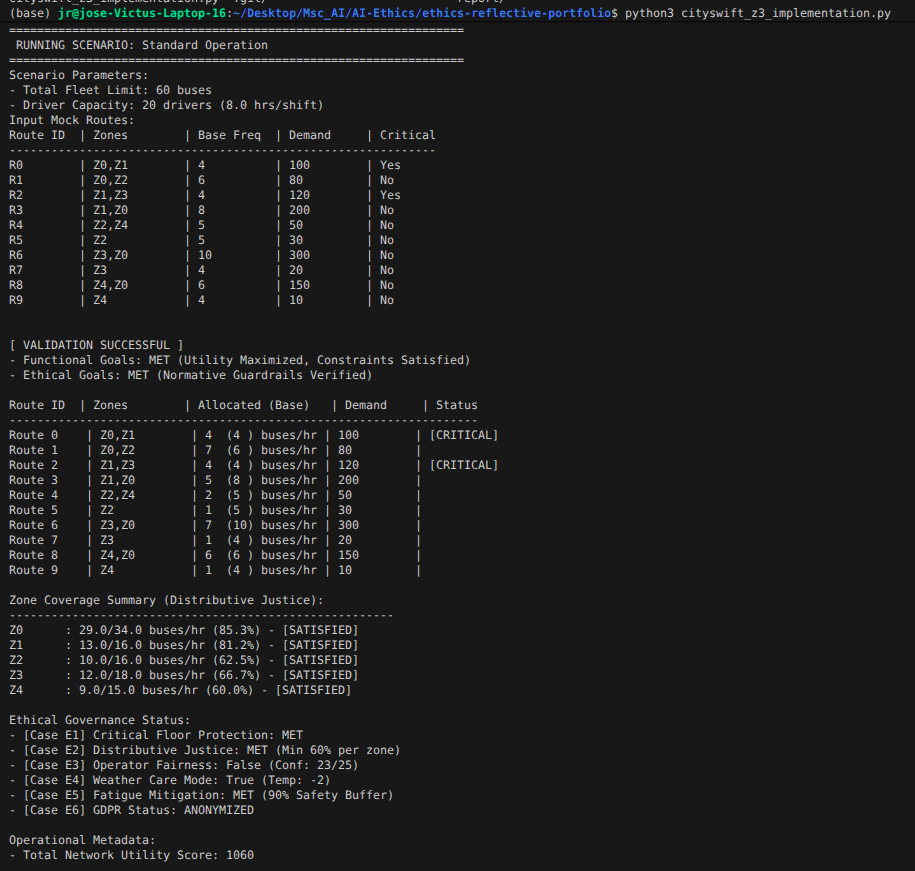
\includegraphics[width=0.95\textwidth]{z3_scenario_success.png}
  \caption{Terminal output showing successful validation of both functional performance and ethical constraint satisfaction.}
  \label{fig:z3_success}
\end{figure}

\subsection{Identification of Goal Unreachability}
As required by the template, Figure \ref{fig:z3_failure} demonstrates the system identifying a situation where goals cannot be reached. In the "Resource Contradiction" scenario, an impossible functional demand is injected, forcing a logical conflict with the ethical safety rules and the operational limits.

\begin{figure}[h!]
  \centering
  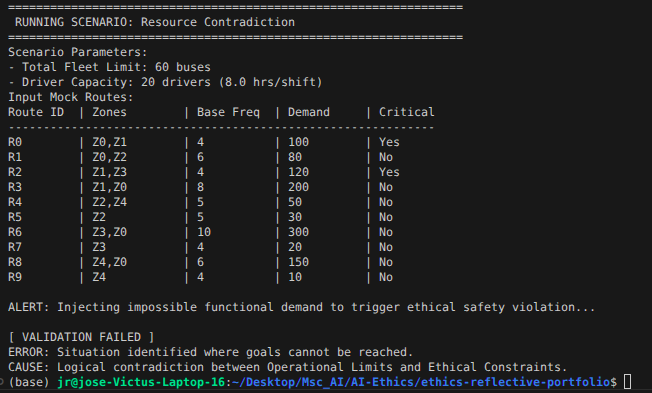
\includegraphics[width=0.95\textwidth]{z3_scenario_failure.png}
  \caption{Terminal output identifying a "Validation Failed" state where functional demands violate ethical safety guardrails.}
  \label{fig:z3_failure}
\end{figure}

\paragraph{Logic Analysis}
The success screenshot (Fig \ref{fig:z3_success}) provides an audit trail showing that the engine maximizes utility while respecting the "Critical" route floors and the sub-zero "Weather Care" mode. Conversely, the failure screenshot (Fig \ref{fig:z3_failure}) proves the solver's robustness: it refuses to generate a plan that would compromise the ethical baseline, correctly flagging a contradiction.

%%%%%%%%
\chapter{ChatGPT Says...}

The version we are going to use for the debates is Gemini 3 Flash, which is the free version available in March 2026

\subsection*{Debate 1: Efficiency vs. Equity (Transit Deserts)}
User:
\begin{figure}[H]aaaaaa
    \centering
    \includegraphics[width=0.8\textwidth]{debate1.png}
\end{figure}
LLM:
c\begin{figure}[H]
    \centering
    \includegraphics[width=0.8\textwidth]{debate1.1.png}
\end{figure}
\begin{figure}[H]
    \centering
    \includegraphics[width=0.8\textwidth]{debate1.2.png}
\end{figure}
\begin{figure}[H]
    \centering
    \includegraphics[width=0.8\textwidth]{debate1.3.png}
\end{figure}

\subsection*{Debate 2: Ecological Stewardship vs. Virtue of Care}
User:
\begin{figure}[H]
    \centering
    \includegraphics[width=0.8\textwidth]{debate2.png}
\end{figure}
LLM:
\begin{figure}[H]
    \centering
    \includegraphics[width=0.8\textwidth]{debate2.1.png}
\end{figure}
\begin{figure}[H]
    \centering
    \includegraphics[width=0.8\textwidth]{debate2.2.png}
\end{figure}
\begin{figure}[H]
    \centering
    \includegraphics[width=0.8\textwidth]{debate2.3.png}
\end{figure}

\subsection*{Debate 3: Algorithmic Transparency vs. Punitive Accuracy}
User:
\begin{figure}[H]
    \centering
    \includegraphics[width=0.8\textwidth]{debate3.png}
\end{figure}
LLM:
\begin{figure}[H]
    \centering
    \includegraphics[width=0.8\textwidth]{debate3.1.png}
\end{figure}
\begin{figure}[H]
    \centering
    \includegraphics[width=0.8\textwidth]{debate3.2.png}
\end{figure}
\begin{figure}[H]
    \centering
    \includegraphics[width=0.8\textwidth]{debate3.3.png}
\end{figure}

\subsection*{Debate 4: Data Privacy vs. Predictive Precision}
User:
\begin{figure}[H]
    \centering
    \includegraphics[width=0.8\textwidth]{debate4.png}
\end{figure}
LLM:
\begin{figure}[H]
    \centering
    \includegraphics[width=0.8\textwidth]{debate4.1.png}
\end{figure}
\begin{figure}[H]
    \centering
    \includegraphics[width=0.8\textwidth]{debate4.2.png}
\end{figure}
\begin{figure}[H]
    \centering
    \includegraphics[width=0.8\textwidth]{debate4.3.png}
\end{figure}

\subsection*{Debate 5: Predictable Reliability vs. Dynamic Throughput}
User:
\begin{figure}[H]
    \centering
    \includegraphics[width=0.8\textwidth]{debate5.png}
\end{figure}
LLM:
\begin{figure}[H]
    \centering
    \includegraphics[width=0.8\textwidth]{debate5.1.png}
\end{figure}
\begin{figure}[H]
    \centering
    \includegraphics[width=0.8\textwidth]{debate5.2.png}
\end{figure}
\begin{figure}[H]
    \centering
    \includegraphics[width=0.8\textwidth]{debate5.3.png}
\end{figure}

\subsection*{Debate 6: Data-Driven Accuracy vs. Worker Safety}
User:
\begin{figure}[H]
    \centering
    \includegraphics[width=0.8\textwidth]{debate6.png}
\end{figure}
LLM:
\begin{figure}[H]
    \centering
    \includegraphics[width=0.8\textwidth]{debate6.1.png}
\end{figure}
\begin{figure}[H]
    \centering
    \includegraphics[width=0.8\textwidth]{debate6.2.png}
\end{figure}
\begin{figure}[H]
    \centering
    \includegraphics[width=0.8\textwidth]{debate6.3.png}
\end{figure}

\chapter{Teammate \#1 Says...}
This chapter is to be written solely by team member \#1\\

Pick \textbf{one} of the cases identified in the previous chapter and argue why the LLM is incorrect. Show a code fragment from your repository to provide evidence for your view.

\textbf{Note:} It is tempting to conclude that the LLM is correct in every case. This usually means that you haven't examined the issue from multiple different perspectives/schools of thought.

\chapter{Teammate \#2 Says...}
This chapter is to be written solely by team member \#2\\

Pick a \textbf{different} case, and argue why the LLM is incorrect. Show a code fragment from your repository,  to provide evidence for your view.


\chapter{Conclusions}
Summarize your thought process about how to approach the ethical cases identified in the second chapter. Which school of ethical thought is easiest for you to express the problem, and find the solution?



%%%%%%%%%%%%%%%%%%%%%%
%%% Acknowledgements
\chapter*{Acknowledgements}

%%%% ADD YOUR BIBLIOGRAPHY HERE



\printbibliography

\end{document}
%\end{article}